
%\begin{figure}[h]
%	\centering
%   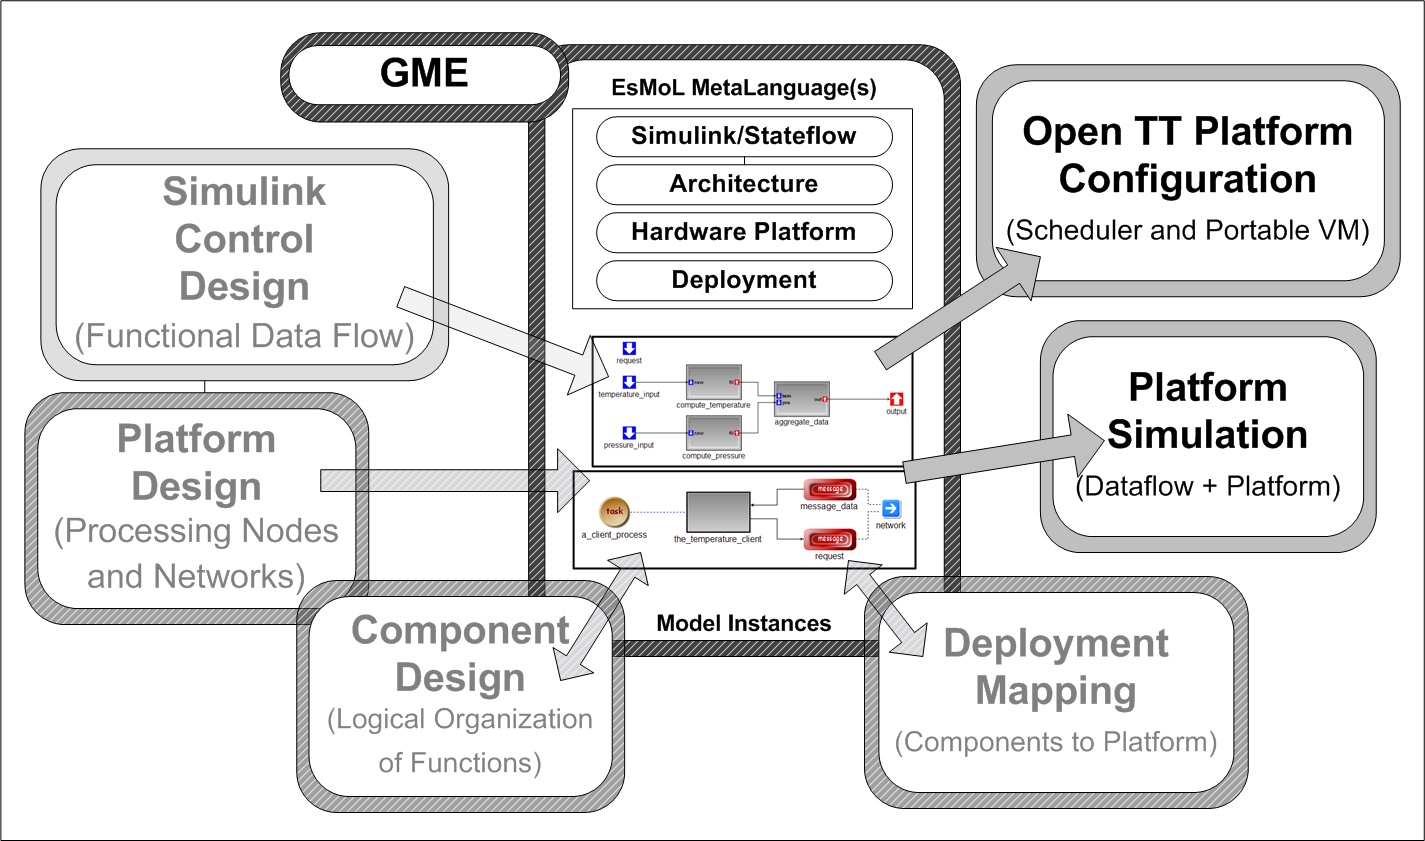
\includegraphics[width=0.55\columnwidth]{diagrams/usecase2.png}
%   \caption{Designers can synthesize simulations which include platform effects. Wrapper and configuration synthesis for time-triggered hardware can also be easily adapted to generate code and configuration for an open time-triggered (TT) platform and related scheduling tools. }
%   \label{fig:uc2}
%\end{figure}

%Fig. \ref{fig:uc2} shows the tool flow for features under development.  
A control system designer initially uses simulation to check correctness of the design.  Software engineers later take code implementing control functions and deploy it to distributed controllers.  Concurrent execution and platform limitations may introduce new behaviors which degrade controller performance and introduce errors.  Ideally, the tools could allow the control functions to be re-simulated with appropriate platform effects.

%\begin{figure}[h]
%	\centering
%   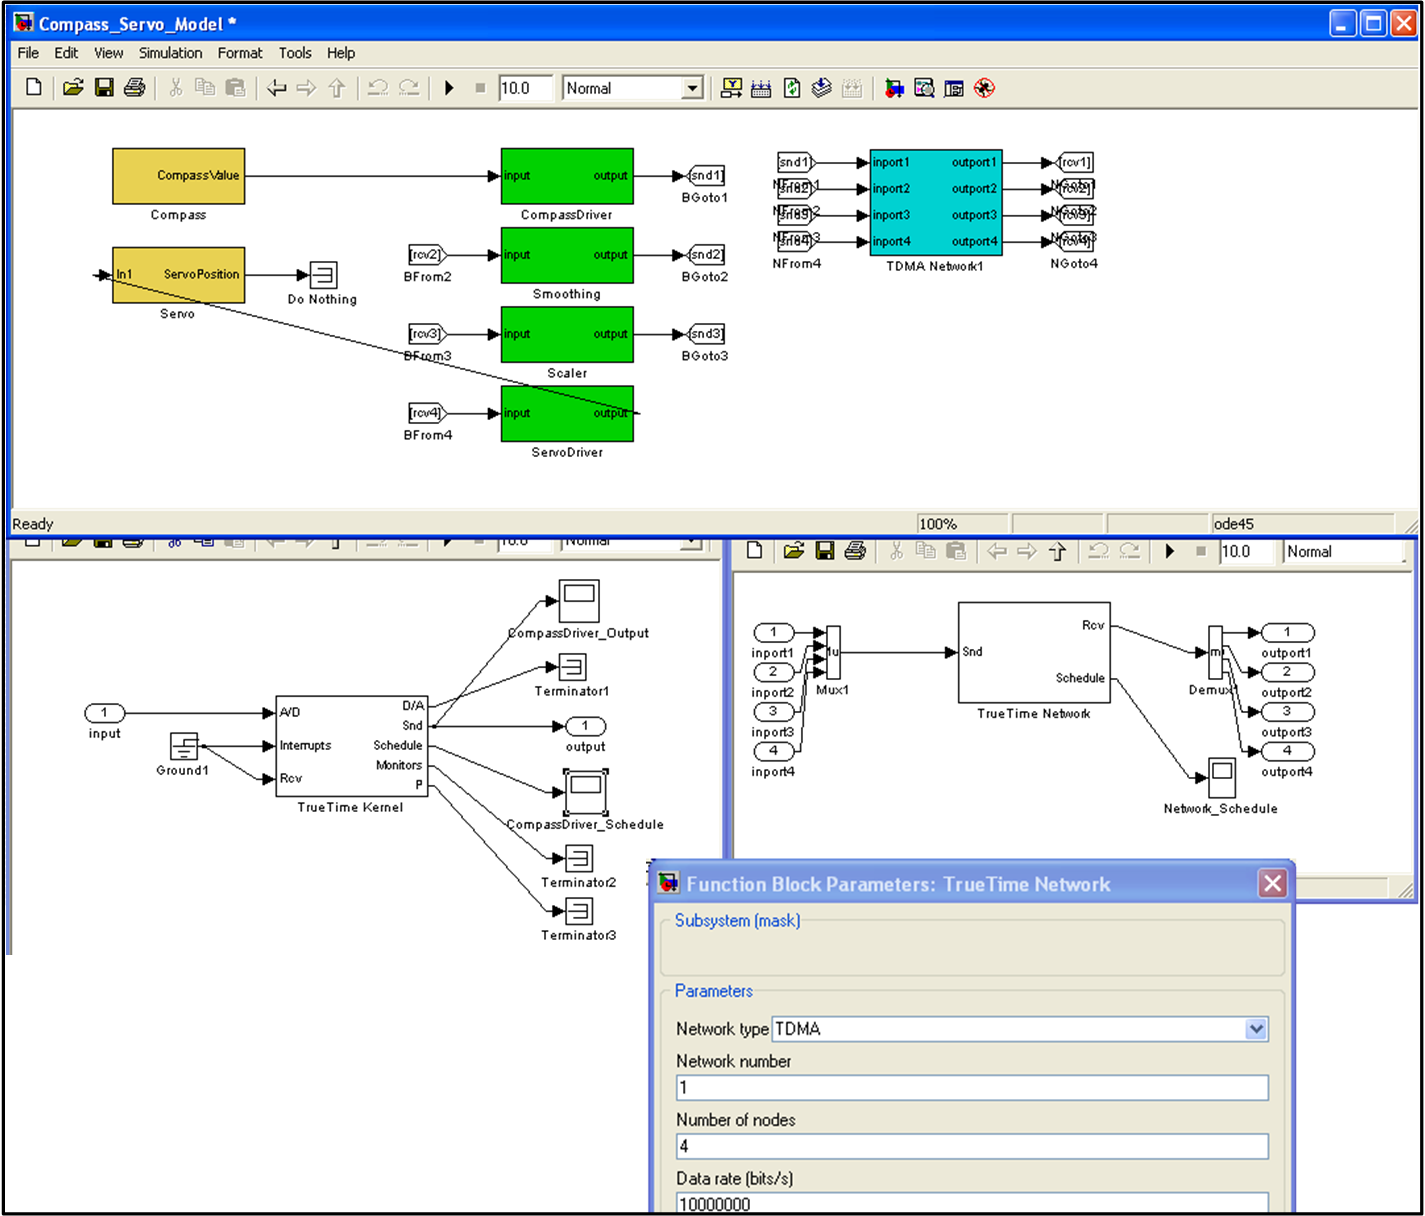
\includegraphics[width=0.5\columnwidth]{diagrams/truetime.png}
%   \caption{TrueTime Simulink model with parameter window.}
%   \label{fig:truetime}
%\end{figure}

The TrueTime simulation environment~\cite{TrueTime} provides Simulink blocks modeling processing nodes and communication links.  Tasks can execute existing C code or invoke subsystems in Simulink models.  Task execution follows configured real-time scheduling models, with communication over a selected medium and protocol.  TrueTime models use a Matlab script to associate platform elements with function implementations.  A platform-specific re-simulation requires this Matlab mapping function, and in our case also a periodic schedule for distributed time-triggered execution.  Both of these can be obtained by synthesis from ESMoL models.  
%Fig. \ref{fig:truetime} shows an example TrueTime model.

After resimulation follows synthesis to a time-triggered platform. In order to use generic computing hardware with this modeling environment, we created a simple, portable time-triggered virtual machine to simulate the timed behavior of a TT cluster~\cite{RT_Thesis} on generic processing hardware.  Since the commercial TT cluster and the open TT virtual machine both implement the same model of computation, synthesis differences amount to management of structural details in the models.  The open VM platform is limited to the timing precision of the underlying processor, operating system, and network, but it is useful for testing.

For both steps above the missing link is schedule generation.  In commercial TTP platforms, associated software tools perform cluster analysis and schedule generation.  For resimulation and deployment to an open platform, an open schedule generation tool is required.  To this end we created a simple schedule generator using the Gecode constraint programming library~\cite{gecode}.  The scheduling approach implements and extends the work of Schild and W{\"u}rtz~\cite{sw:offlinescheduling}.  Configuration for the schedule generator is also generated by the modeling tools.

\subsection{Integration Details}

To configure TrueTime or the scheduler, the important details lie in the deployment model.  Tasks and Messages must be associated with the proper processing nodes and bus channels in the model.  The ISIS UDM libraries~\cite{UDM} provide a portable C++ API for creating interpreters to navigate models and extract the relevant information.  See Fig. \ref{fig:depnew} for the relevant associations.  Model navigation in these intepreters must maintain the relationships between processors and tasks and between buses and messages.  Scheduler configuration also requires extraction of all message sender and receiver dependencies in the model.

%\subsection{Current and Future Work}

%This development stage has had working prototypes and demos for each of the described elements.  The features are being adapted to recent language changes, integrated more fully, and polished.